\documentclass[12pt]{article}
\usepackage[utf8]{inputenc}

\usepackage{lmodern}

\usepackage{enumitem}
\usepackage[margin=2cm]{geometry}

\usepackage{amsmath, amsfonts, amssymb}
\usepackage{graphicx}
%\usepackage{subfigure}
\usepackage{tikz}
\usepackage{pgfplots}
\usepackage{multicol}

\usepackage{comment}
\usepackage{url}
\usepackage{calc}
\usepackage{subcaption}
\usepackage[indent=0pt]{parskip}
\usepackage{animate}

\usepackage{array}
\usepackage{blkarray,booktabs, bigstrut}
\usepackage{bigints}

\pgfplotsset{compat=1.16}

% MATH commands
\newcommand{\ga}{\left\langle}
\newcommand{\da}{\right\rangle}
\newcommand{\oa}{\left\lbrace}
\newcommand{\fa}{\right\rbrace}
\newcommand{\oc}{\left[}
\newcommand{\fc}{\right]}
\newcommand{\op}{\left(}
\newcommand{\fp}{\right)}

\newcommand{\bi}{\mathbf{i}}
\newcommand{\bj}{\mathbf{j}}
\newcommand{\bk}{\mathbf{k}}
\newcommand{\bF}{\mathbf{F}}

\newcommand{\mR}{\mathbb{R}}

\newcommand{\ra}{\rightarrow}
\newcommand{\Ra}{\Rightarrow}

\newcommand{\sech}{\mathrm{sech}\,}
\newcommand{\csch}{\mathrm{csch}\,}
\newcommand{\curl}{\mathrm{curl}\,}
\newcommand{\dive}{\mathrm{div}\,}

\newcommand{\ve}{\varepsilon}
\newcommand{\spc}{\vspace*{0.5cm}}

\DeclareMathOperator{\Ran}{Ran}
\DeclareMathOperator{\Dom}{Dom}

\newcommand{\exo}[1]{\noindent\textcolor{red}{\fbox{\textbf{Problem {#1}}}\hrulefill}\\\\ }
\newcommand{\qu}[4]{\noindent\textcolor{#4}{\fbox{\textbf{Section {#1} | Problem {#2}}} \hrulefill{{\fbox{\textbf{{#3} Points}}}}\\}}

\newcommand{\semester}{Fall 2023}

\newcommand{\CVup}{%

\begin{tikzpicture}
\draw[black, <->, >=latex] (-0.33, 0.5) .. controls (-0.125, 0) and (0.125, 0) .. (0.33, 0.5);
\end{tikzpicture}}

\newcommand{\CVupInc}{%
\begin{tikzpicture}
\draw[black, ->, >=latex] (0,0) .. controls (0.2, 0) and (0.4, 0.2) .. (0.5, 0.5);
\end{tikzpicture}}

\newcommand{\CVupDec}{%
\begin{tikzpicture}[rotate=270]
\draw[black, ->, >=latex] (0,0) .. controls (0.2, 0) and (0.4, 0.2) .. (0.5, 0.5);
\end{tikzpicture}}

\newcommand{\CVdown}{%
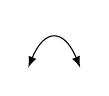
\begin{tikzpicture}
\draw[black, <->, >=latex] (-0.33, -0.5) .. controls (-0.125, 0) and (0.125, 0) .. (0.33, -0.5);
\end{tikzpicture}}

\newcommand{\CVdownInc}{%
\begin{tikzpicture}
\draw[black, ->, >=latex] (-0.5, -0.5) .. controls (-0.5, -0.3) and (-0.5, -0.1) .. (0,0);
\end{tikzpicture}}

\newcommand{\CVdownDec}{%
\begin{tikzpicture}[rotate=-90]
\draw[black, ->, >=latex] (-0.5, -0.5) .. controls (-0.5, -0.3) and (-0.5, -0.1) .. (0,0);
\end{tikzpicture}}

\begin{document}
	\noindent \hrulefill \\
	MATH-244 \semester \hfill Practice Problems Solutions\\
	Section 15.1 \hfill Pierre-Olivier Paris{\'e} \\\vspace*{-1cm}
	
	\noindent\hrulefill
	
	\spc	
	
	\exo{2}
	\\
	According to my lecture notes:
	\begin{enumerate}[label=(\alph*)]
	\item We split the rectangle in 6 smaller rectangles as depicted in the following figure (here $m = 2$ and $n = 3$):
		\begin{center}
		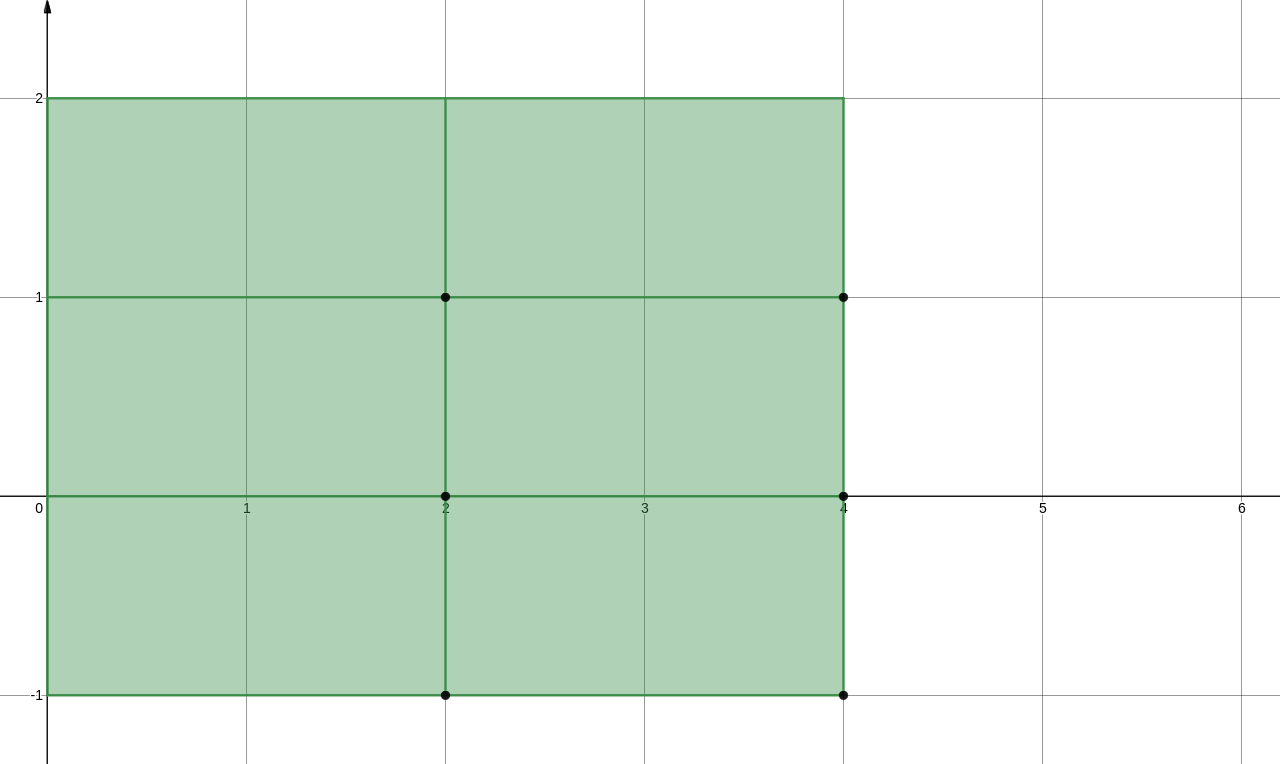
\includegraphics[scale=0.3]{section15-1_Prob2a.png}
		\end{center}
		
		We have $x_1 = 2$, $x_2 = 4$, $y_1 = -1, 0, 2$. We then get
		\begin{align*}
		\iint_R (1 - xy^2 ) \, dA \approx \sum_{i = 1}^2 \sum_{j = 1}^3 (1 - x_i y_j^2) A(R_{ij}) = -12 .
		\end{align*}
	\item We split the rectangle in 6 smaller rectangles as depicted in figure on the next page (here $m = 2$ and $n = 3$):
		
		We have $x_1 = 0, x_2 = 2$, and $y_1 = 0$, $y_2 = 1$, $y_3 = 2$. We then get
		\begin{align*}
		\iint_R (1 - xy^2 ) \, dA \approx \sum_{i = 1}^2 \sum_{j =1}^3 (1 - x_i y_j^2) A(R_{ij}) = -8 .
		\end{align*}
	\begin{center}
		\includegraphics[scale=0.3]{section15-1_Prob2b.png}
		\end{center}
	\end{enumerate}
			
	\spc

	\exo{18}
	\\
	We first compute the inside integral:
		\begin{align*}
		\int_0^{\pi/2} (\sin x + \sin y) \, dy = (y \sin x - \cos y) \Big|_{0}^{\pi/2} = (\pi /2) \sin x + 1 .
		\end{align*}
	Then we can compute the outer integral:
		\begin{align*}
		\int_0^{\pi/6} (\pi/2) \sin x + 1 \, dx = [ - (\pi/2) \cos x + x] \Big|_{0}^{\pi/6} = (8 - 3 \sqrt{3}) \pi/12 \approx 0.734045 .
		\end{align*}

	\spc 

	\exo{32}
	\\
	The integral is over a rectangle, so we use an interated integral. We have
		\begin{align*}
		\iint_R \frac{x}{1 + xy} \, dA = \int_0^1 \int_0^1 \frac{x}{1+x y} \, dy dx .
		\end{align*}
	We put $u = 1 + xy$, so that $du = x dy$. This implies that
		\begin{align*}
		\int_0^1 \frac{x}{1 + xy} \, dy = \int_1^{1 + x} \frac{1}{u} \, du = \ln (1 + x) .
		\end{align*}
	Then, we can evaluate the outer integral:
		\begin{align*}
		\int_0^1 \ln (1 + x) \, dx = 2 ( \ln (2) - 1 ) .
		\end{align*}
	
	\spc
	
	\exo{36}
	\\
	The function $z= 2 - x^2 - y^2$ is a paraboloide that is going downward and that is 2 units above the XY-plane. We are also integrating on the square $R = [0, 1] \times [0, 1]$. So the solid should look like this:
		\begin{center}
		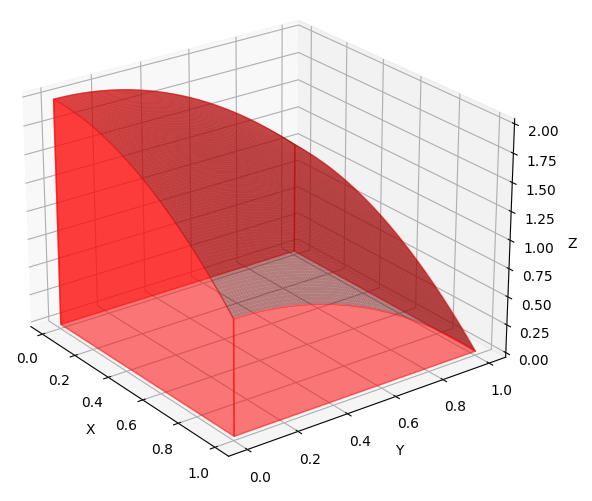
\includegraphics[scale=0.42]{Prob36-Pic2.png}
		\end{center}
	
	
\end{document}